\documentclass[12pt]{article}
%Page set up
\setlength{\topmargin}{-1in}
\setlength{\textwidth}{7in}
\setlength{\oddsidemargin}{-.25in}
\setlength{\textheight}{9.5in}
%Shortcuts
\def\it{\item}
\def\ul#1{\underline{#1}} \def\spul{\underline{\hspace{.75in}}} \def\ol#1{\overline{#1}}
\def\sspul{\ \underline{\hspace{.25in}} \ } \def\blank{\ul{\h{1.5}}}
\def\v#1{\vspace{#1in}} \def\h#1{\hspace{#1in}}
\def\be{\begin{enumerate}} \def\ee{\end{enumerate}}
\def\bc{\begin{center}} \def\ec{\end{center}}
\def\bd{\begin{description}} \def\ed{\end{description}}
\def\bt{\begin{tabular}} \def\et{\end{tabular}}
\def\lp{\left(} \def\rp{\right)} \def\abs#1{\vert #1 \vert}
\def\bar#1{\overline{#1}}
%General Math
\def\dis{\displaystyle}
\def\Frac#1#2{\displaystyle{\frac{#1}{#2}}}
\def\rta{\rightarrow}
\def\inv#1{{#1}^{-1}} % inverse of arg 
\def\th{\theta} \def\al{\alpha} \def\ba{\beta} \def\ga{\gamma}
\def\R{\mathbb{R}} \def\Q{\mathbb{Q}} \def\N{\mathbb{N}} \def\Z{\mathbb{Z}} \def\P{\mathbb{P}}
\def\X{\mathbb{X}} \def\Y{\mathbb{Y}} \def\U{\mathbb{U}} \def\E{\mathbb{E}} \def\C{\mathbb{C}}
\def\F{\mathbb{F}}
\def\mtrx#1{\begin{pmatrix}
#1_{11} & #1_{12} & \cdots & #1_{1n} \\
#1_{21} & #1_{22} & \cdots & #1_{2n} \\
\vdots & \vdots & \ddots & \vdots \\
#1_{m1} & #1_{m2} & \cdots & #1_{mn}
\end{pmatrix} }
\def\Idd{\begin{pmatrix} 1 & 0 \\ 0 & 1 \end{pmatrix}}
\def\Iddd{\begin{pmatrix} 1 & 0 & 0 \\ 0 & 1 & 0 \\ 0 & 0 & 1 \end{pmatrix}}
\def\colt#1#2{\lp \begin{array}{rr} #1 \\ #2 \end{array} \rp}
\def\colth#1#2#3{\lp \begin{array}{rrr} #1 \\ #2 \\ #3 \end{array} \rp}
\def\colf#1#2#3#4{\lp \begin{array}{rrrr} #1 \\ #2 \\ #3 \\ #4 \end{array} \rp}
\def\colp#1{\begin{pmatrix} #1_1 \\ #1_2 \\ \vdots \\ #1_p \end{pmatrix}}
\def\colm#1{\begin{pmatrix} #1_1 \\ #1_2 \\ \vdots \\ #1_m \end{pmatrix}}
\def\coln#1{\begin{pmatrix} #1_1 \\ #1_2 \\ \vdots \\ #1_n \end{pmatrix}}
\def\rowp#1{\begin{pmatrix} #1_1 & #1_2 & \cdots & #1_p \end{pmatrix}}
\def\rowt#1#2{\begin{pmatrix} #1 & #2 \end{pmatrix}}
\def\rowth#1#2#3{\begin{pmatrix} #1 & #2 & #3 \end{pmatrix}}
\def\rowf#1#2#3#4{\begin{pmatrix} #1 & #2 & #3 & #4 \end{pmatrix}}
\def\bfourt{\begin{tabbing}
xxxxxxxxxxxxxxxxxx \=
xxxxxxxxxxxxxxxxxx \=
xxxxxxxxxxxxxxxxxx \=
xxxxxxxxxxxxxxxxxx \kill}
\def\bttt{\begin{tabbing}
xxxxxxxxxxxxxxxxxxxxxxxxxxxxx \=
xxxxxxxxxxxxxxxxxxxxxxxxxxxxx \=
xxxxxxxxxxxxxxxxxxxxxxxxxxxxx \kill}
\def\btt{\begin{tabbing}
xxxxxxxxxxxxxxxxxxxxxxxxxxxxxxxxxxxxxxxxx \=
xxxxxxxxxxxxxxxxxxxxxxxxxxxxx \kill}
\def\etb{\end{tabbing}}
% cú pháp: Định nghĩa i: nội dung
\newtheorem{thm}{Định nghĩa}
\newtheorem{ex}[thm]{VD}
\newenvironment{linsys}[2][m]{%
\setlength{\arraycolsep}{.1111em} % p. 170 TeXbook; a medmuskip
\begin{array}[#1]{@{}*{#2}{rc}r@{}} 
}{%
\end{array}}

\usepackage{amssymb,amsmath,pstricks,framed}
\usepackage[vietnamese]{babel}
\usepackage{amsmath}
\usepackage[utf8]{inputenc}
\usepackage[T1]{fontenc}
\usepackage{graphicx}
\usepackage{color}
\usepackage{hyperref}

\setcounter{page}{1}
\begin{document}

% những nội dung cơ bản về môn xác suất thống kê
% tiêu đề, không chứa ngày tháng
\title{Xác suất thống kê}
\date{}
\maketitle
% nội dung
% phần 1: Công thức xác suất
% phần 2: Hàm mật độ xác suất, hàm phân phối xác suất
% phần 3: Phân phối nhị thức
% phần 4: Phân phối poisson
% phần 5: Phân phối chuẩn
% phần 6: Các dạng bài toán xác suất thống kê
% phần 7: Bảng giá trị

\section{Công thức xác suất}
\subsection{Kiến thức cơ bản}
% định nghĩa : P(A) = xác suất của biến cố A
\begin{thm}
$P(A)$ được gọi là xác suất của biến cố A
\begin{equation}
    P(A + B) = P( A \cup B) 
\end{equation}
\begin{equation}
    P(A)P(B) = P(A \cap B) 
 \end{equation}0
\begin{equation}
    P(A + B) = P(A) + P(B) - P(AB)
    \end{equation}
Nếu A B xung khắc:
\begin{equation}
P(A + B) = P(A) + P(B) 
\end{equation}
\end{thm}

\begin{thm}
Xác suất biến cố đối của A là xác suất không xảy ra A
\begin{equation}
P(\bar{A}) = 1 - P(A)
\end{equation}
\end{thm}
\begin{thm}
\begin{equation}
    P(AB) = P(A)P(B)
\end{equation}
\end{thm}

\begin{thm}
Nếu A B không độc lập
\begin{equation}
    P(AB) = P(B|A)P(A) = P(A|B)P(B) = P(A) + P(B) - P(A + B)
\end{equation}
\end{thm}

\subsection{Xác suất có điều kiện}
\begin{thm}
Xác suất của biến cố A khi biết biến cố B đã xảy ra
\begin{equation}
P(A|B) = \frac{P(AB)}{P(B)}
\end{equation}
Từ đó có công thức
\begin{equation}
P(AB) = P(A|B)P(B) = P(B|A)P(A)
\end{equation}
Với 3 biến cố A B C
\begin{equation}
P(ABC) = P(A|BC)P(BC) = P(B|AC)P(AC) = P(C|AB)P(AB)
\end{equation}
\end{thm}

\begin{thm}
Công thức xác suất toàn phần
\begin{equation}
P(F) = \sum_{i=1}^n P(F|A_i)P(A_i)
\end{equation}
Hay ta có thể viết lại
\begin{equation}
P(F) = P(F|A_1)P(A_1) + P(F|A_2)P(A_2) + \cdots + P(F|A_n)P(A_n)
\end{equation}
\end{thm}

\begin{thm}
Công thức Bayes
\begin{equation}
P(A_i|F) = \frac{P(F|A_i)P(A_i)}{P(F)}
\end{equation}
Mở rộng cho 3 biến cố A, B C độc lập:
\begin{equation}
P(A|BC) = \frac{P(BC|A)P(A)}{P(BC)} = \frac{P(B|A) P(C|A) P(A)}{P(B)P(C)}
\end{equation}
Trường hợp $A, B_1 = B_2 = ... = B_n$:
\begin{equation}
P(A|B_1B_2...B_n) = \frac{P(B|A)^n P(A)}{P(B)^n}
\end{equation}
\end{thm}

\begin{thm}
    Chứng minh biến cố A B độc lập, ta cần chứng minh 1 trong 2 cách sau:
    \begin{enumerate}
        \item $P(AB) = P(A)P(B)$
        \item $P(A|B) = P(A)$ hoặc $P(B|A) = P(B)$
    \end{enumerate}
    Lưu ý: $P(A+B) = P(A) + P(B)$ không phải là điều kiện để A B độc lập \\
    phải tìm $P(AB)$ từ $P(AB) = P(A)P(B) - P(A+B)$, rồi kiểm tra như trên

\end{thm}

\subsection{Công thức Bernoulli}

\begin{thm}
Xác suất của biến cố A xảy ra k lần trong n lần thử là:
\begin{equation}
P(A) = C_n^k p^k (1-p)^{n-k}
\end{equation}
\end{thm}

\section{Hàm phân phối xác suất, hàm mật độ xác suất}
\subsection{Hàm phân phối xác suất}
\begin{thm}
Hàm phân phối xác suất của biến ngẫu nhiên rời rạc X có dạng
\end{thm}
% table of probability distribution function
\begin{tabular}{|c|c|}
    \hline
    $X$ & $x_1$, $x_2$, $\cdots$, $x_n$ \\
    \hline
    $P(X)$ & $p_1$, $p_2$, $\cdots$, $p_n$ \\
    \hline
  \end{tabular}
\begin{thm}
    Kỳ vọng:
    \begin{equation}
    E(X) = \sum_{i=1}^n x_ip_i = x_1p_1 + x_2p_2 + \cdots + x_np_n
    \end{equation}
    \begin{equation}
    E(X^2) = \sum_{i=1}^n x_i^2p_i = x_1^2p_1 + x_2^2p_2 + \cdots + x_n^2p_n
    \end{equation}
    Phương sai:
    \begin{equation}
    Var(X) = E(X^2) - E(X)^2
    \end{equation}
    Độ lệch chuẩn:
    \begin{equation}
    \sigma = \sqrt{Var(X)}
    \end{equation}
\end{thm}


\subsection{Hàm mật độ xác suất}
\begin{thm}
Hàm mật độ xác suất của biến ngẫu nhiên liên tục X có dạng
\begin {equation}
% tích phân từ trừ vô cùng đến cộng vô cùng fx = 1
\int_{-\infty}^{\infty} f(x)dx = 1
\end{equation}
\begin {equation}
% biểu diễn dưới dạng liệt kê
f(x) = \begin{cases}
p_1, & x = x_1 \\
p_2, & x = x_2 \\
\vdots, & \vdots \\
p_n, & x = x_n \\
0, & \text{otherwise}
\end{cases}
\end{equation}
\begin {equation}
P(a \leq X \leq b) = \int_a^b f(x)dx
\end{equation}
\begin {equation}
P(X > a) = 1 - \int_{-\infty}^a f(x)dx = \int_a^{\infty} f(x)dx
\end{equation}
\begin {equation}
P(X < a) = \int_{-\infty}^a f(x)dx
\end{equation}
\end{thm}

\begin {thm}
Cách tìm hằng số chuẩn hóa
\begin {equation}
1 = \int_{-\infty}^{\infty} Cf(x)dx = C\int_a^b f(x)dx = CF(x)|^b_a = CF(b) - CF(a)
\end{equation}
hoặc đơn giản hơn:
\begin{equation}
    C = \frac{1}{\int_{-\infty}^{\infty}f(x)dx} = \frac{1}{\int_{a}^{b}f(x)dx}
\end{equation}
\end{thm}

\begin{thm}
    Xác suất có điều kiện trong trường hợp biến ngẫu nhiên liên tục:
    \begin{equation}
    P(A|B) = \frac{\int_{A \cap B} f(x)dx}{\int_B f(x)dx}
    \end{equation}
\end{thm}
\begin{ex}
    Xác suất để $x \geq 4$ khi $x$ đã $\geq 2$
    \begin{equation}
    P(x \geq 4 | x \geq 2) = \frac{P(x \geq 4 \cap x \geq 2)}{P(x \geq 2)} = \frac{\int_{x \geq 4 \cap x \geq 2} f(x)dx}{\int_{x \geq 2} f(x)dx} = \frac{\int_{4}^{\infty} f(x)dx}{\int_{2}^{\infty} f(x)dx}
    \end{equation}
\end{ex}

\begin{thm}
    Kỳ vọng:
    \begin{equation}
    E(X) = \int_{-\infty}^{\infty} xf(x)dx
    \end{equation}
    \begin{equation}
    E(X^2) = \int_{-\infty}^{\infty} x^2f(x)dx
    \end{equation}
    Phương sai:
    \begin{equation}
    Var(X) = E(X^2) - E(X)^2
    \end{equation}
    Độ lệch chuẩn:
    \begin{equation}
    \sigma = \sqrt{Var(X)}
    \end{equation}
\end{thm}

\begin{thm}
    Hàm phân phối xác suất của biến ngẫu nhiên liên tục X có dạng
    \begin{equation}
    F(x) = P(X \leq x) = \int_{-\infty}^x f(t)dt
    \end{equation}
    \begin{equation}
    F(x) = \begin{cases}
    0, & x < a \\
    \frac{x-a}{b-a}, & a \leq x \leq b \\
    1, & x > b
    \end{cases}
    \end{equation}
    Tính trực tiếp xác suất từ hàm phân phối xác suất:
    \begin{equation}
    P(a \leq X \leq b) = F(b) - F(a)
    \end{equation}
    \begin{equation}
    P(X > a) = 1 - F(a)
    \end{equation}
    \begin{equation}
    P(X < a) = F(a)
    \end{equation}
\end{thm}

\begin{thm}
    Định lý Chebysev: cho $X$ là biến ngẫu nhiên có kỳ vọng $E(X) = \mu$ và phương sai $Var(X) = \sigma^2$. Khi đó:
    \begin{equation}
    P(|X - \mu| \geq \epsilon) \leq \frac{\sigma^2}{\epsilon^2}
    \end{equation}
    \begin{equation}
        P(\mu - \epsilon \leq X \leq \mu + \epsilon) \geq 1 - \frac{\sigma^2}{\epsilon^2}
    \end{equation}
\end{thm}

\begin{thm}
    Trung vị: giá trị biến ngẫu nhiên X sao cho $P(X \leq x) = 0.5$
    \begin{equation}
    \int_{-\infty}^x f(t)dt = 0.5
    \end{equation}
\end{thm}

\section{Các phân phối xác suất thường gặp}
\subsection{Phân phối Bernoulli}
\begin{thm}
    Một phép thử Bernoulli là một phép thử chỉ có hai kết quả có thể xảy ra: thành công A hoặc thất bại $\bar{A}$, trong đó $P(A) = p$ và $P(\bar{A}) = 1 - p$.
    Phân phối Bernoulli: Ký hiệu $X \sim B(p)$, khi đó:
    \begin{equation}
    f(x) = \begin{cases}
    p, & x = 1 \\
    1 - p, & x = 0
    \end{cases}
    \end{equation}
    \begin{equation}
    F(x) = \begin{cases}
        p & x = 1 \\
        1 - p & x = 0 \\
        0 & \text{otherwise}
    \end{cases}
    \end{equation}
    \begin{equation}
    P(X = 1) = p
    \end{equation}
    \begin {equation}
    P(X = 0) = 1 - p
    \end{equation}
    \begin{equation}
    E(X) = p
    \end{equation}
    \begin{equation}
    Var(X) = p(1 - p)
    \end{equation}
\end{thm}

\subsection{Phân phối nhị thức}
\begin{thm}
    Phân phối nhị thức: là phân phối của một biến ngẫu nhiên mà nó là số lần thành công trong một dãy n phép thử Bernoulli độc lập với nhau. Ký hiệu $X \sim B(n, p)$, khi đó:
    n là số lần thử, p là xác suất thành công của mỗi lần thử.
    
    \begin{equation}
    f(x) = \begin{cases}
        C_n^x p^x(1-p)^{n-x}, & x = 0, 1, \dots, n \\
    0, & \text{otherwise}
    \end{cases}
    \end{equation}
    \begin{equation}
    F(x) = \begin{cases}
    \sum_{i=0}^x C_n^i p^i(1-p)^{n-i}, & x = 0, 1, \dots, n \\
    0, & \text{otherwise}
    \end{cases}
    \end{equation}
    \begin{equation}
        P(X = k) = C_n^k p^k(1-p)^{n-k}
    \end{equation}
    \begin{equation}
        P(X \geq k) = \sum_{i=k}^n C_n^i p^i(1-p)^{n-i}
    \end{equation}
    \begin{equation}
        P(X \leq k) = \sum_{i=0}^k C_n^i p^i(1-p)^{n-i}
    \end{equation}

    \begin{equation}
    E(X) = np
    \end{equation}
    \begin{equation}
    Var(X) = np(1 - p)
    \end{equation}
\end{thm}

\begin{thm}
    Chuyển từ phân phối nhị thức sang phân phối Poisson:
    \begin{equation}
    B(n, p) \sim P(\lambda), \text{ với } \lambda = np
    \end{equation}

\end{thm}
\begin{thm}
    Chuyển từ phân phối nhị thức sang phân phối chuẩn:
    \begin{equation}
    B(n, p) \sim N(\mu, \sigma^2), \text{ với } \mu = np, \sigma^2 = np(1 - p)
    \end{equation}

\end{thm}
 
\subsection{Phân phối siêu bội}
\begin{thm}
    Xét tập N trong đó có M phần tử có tính chất P và N-M phần tử không có tính chất P. 
    Chọn k phần tử khác nhau không phân biệt từ N phần tử. 
    Gọi X là số phần tử có tính chất P trong k phần tử đã chọn. 
    X có phân phối siêu bội với 3 tham số N, M, n. 
    Ký hiệu $X \sim H(N, M, n)$, khi đó:
    \begin{equation}
        P(X = k) = \frac{C_M^k C_{N-M}^{n-k}}{C_N^n}
    \end{equation}
    \begin{equation}
        P(X \geq k) = \sum_{i=k}^n \frac{C_M^i C_{N-M}^{n-i}}{C_N^n}
    \end{equation}
    \begin{equation}
        P(X \leq k) = \sum_{i=0}^k \frac{C_M^i C_{N-M}^{n-i}}{C_N^n}
    \end{equation}
    \begin{equation}
        E(X) = \frac{Mn}{N}
    \end{equation}
    \begin{equation}
        Var(X) = \frac{N-n}{N-1}n\frac{M}{N}(1 - \frac{M}{N})
    \end{equation}
\end{thm}
\begin{thm}
    Chuyển từ phân phối siêu bội sang phân phối nhị thức:
    \begin{equation}
    H(N, M, n) \sim B(n, \frac{M}{N})
    \end{equation}
\end{thm}

\subsection{Phân phối Poisson}
\begin{thm}
    Phân phối Poisson: là phân phối của một biến ngẫu nhiên mà nó là số lần xảy ra của một sự kiện trong một khoảng thời gian hoặc không gian nhất định. Ký hiệu $X \sim P(\lambda)$, với $\lambda$ là trung bình số lần xuất hiện biến cố, khi đó:
    \begin{equation}
        P(X = k) = \frac{e^{-\lambda}\lambda^k}{k!}, k = 0, 1, 2, \dots
    \end{equation}
    \begin{equation}
        P(X \geq k) = \sum_{i=k}^{\infty} \frac{e^{-\lambda}\lambda^i}{i!} = 1 - \sum_{i=0}^{k-1} \frac{e^{-\lambda}\lambda^i}{i!}
    \end{equation}
    \begin{equation}
        P(X \leq k) = \sum_{i=0}^{k} \frac{e^{-\lambda}\lambda^i}{i!}
    \end{equation}
    \begin{equation}
        P(a \leq X \leq b) = \sum_{i=a}^{b} \frac{e^{-\lambda}\lambda^i}{i!}
    \end{equation}
    \begin{equation}
        E(X) = \lambda
    \end{equation}
    \begin{equation}
        Var(X) = \lambda
    \end{equation}
\end{thm}
\begin{thm}
    Chuyển từ phân phối poisson sang phân phối chuẩn:
    \begin{equation}
    P(\lambda) \sim N(\mu, \sigma^2), \text{ với } \mu = \lambda, \sigma^2 = \lambda
    \end{equation}

\end{thm}

\subsection{Phân phối chuẩn}
\begin{thm}
    Phân phối chuẩn: là phân phối của một biến ngẫu nhiên mà nó là tổng của nhiều biến ngẫu nhiên độc lập với nhau. Ký hiệu $X \sim N(\mu, \sigma^2)$, khi đó:
    \begin{equation}
        f(x) = \frac{1}{\sqrt{2\pi}\sigma}e^{-\frac{(x - \mu)^2}{2\sigma^2}}
    \end{equation}
    \begin{equation}
        E(X) = \mu
    \end{equation}
    \begin{equation}
        Var(X) = \sigma^2
    \end{equation}
\end{thm}

\begin{thm}
    Phân phối chuẩn tắc: là phân phối chuẩn với $\mu = 0, \sigma = 1$ Ký hiệu $X \sim N(0, 1)$, khi đó:
    \begin{equation}
        f(x) = \frac{1}{\sqrt{2\pi}}e^{-\frac{x^2}{2}}
    \end{equation}
\end{thm}
\begin{thm}
    Đổi biến từ phân phối chuẩn sang phân phối chuẩn tắc:
    \begin{equation}
        X \sim N(\mu, \sigma^2) \rightarrow Z = \frac{X - \mu}{\sigma} \sim N(0, 1)
    \end{equation}
    Khi đó:
    \begin{equation}
        P(X \leq b) = P(Z \leq \frac{b - \mu}{\sigma}) = \Phi(\frac{b - \mu}{\sigma})
    \end{equation}
    \begin{equation}
        P(X \geq a) = 1 - \Phi(\frac{a - \mu}{\sigma})
    \end{equation}
    \begin{equation}
        P(a \leq X \leq b) = \Phi(\frac{b - \mu}{\sigma}) - \Phi(\frac{a - \mu}{\sigma})
    \end{equation}
    Cách tính $\Phi(z)$:
    \begin{equation}
        \Phi(z) = \int_{-\infty}^z \frac{1}{\sqrt{2\pi}}e^{-\frac{t^2}{2}}dt = \frac{1}{2} + \int_{0}^z \frac{1}{\sqrt{2\pi}}e^{-\frac{t^2}{2}}dt
    \end{equation}
    Do $\frac{1}{2}$ bị triệt tiêu, nên:
    \begin{equation}
        \Phi(B) - \Phi(A) = \int_{0}^b \frac{1}{\sqrt{2\pi}}e^{-\frac{t^2}{2}}dt - \int_{0}^a \frac{1}{\sqrt{2\pi}}e^{-\frac{t^2}{2}}dt = \int_{a}^b \frac{1}{\sqrt{2\pi}}e^{-\frac{t^2}{2}}dt
    \end{equation}
    Hoặc xem bảng giá trị \ref{fig:nd1} và \ref{fig:nd2}
\end{thm}

\begin{thm}
    Dùng hiệu chỉnh liên tục để tính xác xuất $P(X =a)$:
    \begin{equation}
        P(X = a) \approx P(a - \frac{1}{2} < X < a + \frac{1}{2}) \approx \Phi(\frac{a + \frac{1}{2} - \mu}{\sigma}) - \Phi(\frac{a - \frac{1}{2} - \mu}{\sigma})
    \end{equation}
    Dùng hiệu chỉnh rời rạc để tính xác xuất $P( a \leq X \leq b)$:
    \begin{equation}
        P(a \leq X \leq b) \approx P(a - \frac{1}{2} < X < b + \frac{1}{2}) \approx \Phi(\frac{b + \frac{1}{2} - \mu}{\sigma}) - \Phi(\frac{a - \frac{1}{2} - \mu}{\sigma})
    \end{equation}

\end{thm}

\begin{thm}
    Chuyển từ phân phối chuẩn sang phân phối nhị thức:
    \begin{equation}
        N(\mu, \sigma^2) \sim B(n, p) \text{ với } p = \frac{\mu}{\sigma^2}, n = \frac{\sigma^2}{p(1 - p)}
    \end{equation}

\end{thm}

\section {Các dạng toán thường gặp}
\subsection{Dàn ý giải 1 bài toán bất kỳ}
\begin{enumerate}
    \item Xác định loại bài toán: nếu là xác suất, thì là xác suất độc lập hay xác suất có điều kiện? \\
    nếu là phân phối, thì phân phối gì?
    \item Xác định yêu cầu bài toán: bài toán hỏi gì? công thức cuối cùng cần tìm là gì?
    \item Phân tích thành phần bài toán:
    gọi tên các biến cố bằng ký hiệu, tính xác suất các biến cố đó
    \item Tìm công thức cần tính
\end{enumerate}

\subsection{Dấu hiệu của các phân phối}
Phân phối nhị thức: số lượng + xác suất \\
Phân phối Poisson: số lượng + thời gian \\
Phân phối chuẩn: kỳ vọng (trung bình) + độ lệch chuẩn \\

\subsection{Một số ví dụ}
Ví dụ: Trong một cửa hiệu kinh doanh điện thoại di động, tỉ lệ điện
thoại di động của hãng Nokia, Samsung và Iphone lần lượt là 20\%, 50\% và 30\%. Tỉ
lệ bị trục trặc (về cài đặt) trong thời gian bảo hành của các loại diện thoại di động
của hãng Nokia, Samsung và Iphone tương ứng là 6\%, 8\%, 7\%. Giả sử một khách
hàng mua ngẫu nhiên một điện thoại di động và điện thoại đó không bị trục trặc
trong suốt thời gian bảo hành. Tính xác suất để điện thoại đó của hãng Samsung.
\begin{enumerate}
    \item Xác định loại bài toán: Bài toán thuộc loại xác suất có điều kiện.
    \item Xác định yêu cầu bài toán: Tìm xác suất để điện thoại đó của hãng Samsung mà không bị trục trặc trong suốt thời gian bảo hành.
    \item Phân tích thành phần bài toán:
    \subitem Gọi $X$ là biến cố điện thoại trục trặc trong suốt thời gian bảo hành.
    \subitem Gọi $N$, $S$, $I$ lần lượt là biến cố điện thoại của hãng Nokia, Samsung, Iphone. \\ $P(N) = 0.2$, $P(S) = 0.5$, $P(I) = 0.3$.
    \\ $P(X|N) = 0.06$, $P(X|S) = 0.08$, $P(X|I) = 0.07$.
    \item Tìm xác suất cần tính: \\
    $P(X) = P(X|N)P(N) + P(X|S)P(S) + P(X|I)P(I) = 0.06 . 0.2 + 0.08 . 0.5 + 0.07 . 0.3 = 0.073$ \\
    $P(S|\bar{X}) = \frac{P(S)P(\bar{X}|S)}{1-P(X)} = \frac{0.5 . 0.92}{1-0.073} = 0.496$

\end{enumerate}
Ví dụ: Một nhà máy dệt có 1000 ống sợi. Xác suất để trong 1 giờ máy
hoạt động có 1 ống sợi bị đứt là 0.002. Tính xác suất để trong 1 giờ máy hoạt động
có không quá 4 ống sợi bị đứt.

\begin{enumerate}
    \item Xác định loại bài toán: Bài toán có thể quy về phân phối nhị thức
    \item Xác định yêu cầu bài toán: Tính xác suất để trong 1 giờ máy hoạt động có không quá 4 ống sợi bị đứt.
    \item Phân tích thành phần bài toán:
    \subitem Gọi $X$ là số ống sợi bị đứt trong 1 giờ máy hoạt động.
    \\ $X \sim B(n, p), n = 1000, p = 0.002$
    \item Tìm xác suất cần tính: \\
    $P(X \leq 4) = \sum_{k=0}^{4} C_{n}^{k} p^k (1-p)^{n-k} = 0.9475$ \\
    Hoặc tính xấp xỉ bằng phân phối Poisson: \\
    $X \sim P(\lambda), \lambda = np = 2$ \\
    $P(X \leq 4) = \sum_{k=0}^{4} \frac{e^{-\lambda} \lambda^k}{k!} = 0.9475$

\end{enumerate}
Ví dụ: Thời gian tải một tập tin có dung lượng dưới 20MB từ một
website được mô hình hóa bởi biến ngẫu nhiên X (tính theo phút) có hàm mật độ
như sau:
\begin{equation}
    f(x) = \begin{cases}
        C(5x^3-x^4) & x \in [0, 5] \\
        0, & \text{otherwise}
    \end{cases}
\end{equation}
a. Xác định C. \\
b. Tính thời gian trung bình để tải một tập tin có dung lượng dưới 20MB từ
website đó. \\
c. Giả sử bạn thấy tập tin đó vẫn chưa tải xong sau khi bắt đầu tải được 2
phút. Tính xác suất phải mất hơn 2 phút nữa mới tải xong tập tin.

\begin{enumerate}
    \item Xác định loại bài toán: Bài toán liên quan đến hàm mật độ xác suất.
    \item a. Ta có: \\
    $\int_{-\infty}^{\infty} f(x)dx = \int_{0}^{5} C(5x^3-x^4) dx = 1$ \\
    $C = \frac{1}{\int_{0}^{5} 5x^3-x^4 dx} = \frac{4}{625}$ \\
    b. $E(X) = \int_{-\infty}^{\infty} xf(x)dx = \int_{0}^{5} \frac{4}{625}x(5x^3-x^4) dx = \frac{10}{3}$ \\
    c. $P(X > 4 | X > 2) = \frac{P(X > 4)}{P(X > 2)} = \frac{\int_{4}^{5} \frac{4}{625}(5x^3-x^4) dx}{\int_{2}^{5} \frac{4}{625}(5x^3-x^4) dx} = 0.2875$
\end{enumerate}
Ví dụ: Giả sử nồng độ chloride trong máu (mmol/L) có phân phối
chuẩn với trung bình là 104 và độ lệch chuẩn là 5.
a. Tính tỉ lệ người có nồng độ chloride trong máu nhiều hơn 105.
b. Chọn ngẫu nhiên 1000 người. Tính xác suất có từ 200 đến 300 người có nồng
độ chloride trong máu nhiều hơn 105.
\begin{enumerate}
    \item Xác định loại bài toán: Bài toán có thể quy về phân phối chuẩn. \\
    Gọi X là nồng độ chloride trong máu. \\
    $X \sim N(\mu, \sigma^2), \mu = 104, \sigma = 5$
    \item a. $P(X > 105) = 1 - \Phi(\frac{105-104}{5}) = 0.4207$ \\
    b. Gọi $Y$ là số người có nồng độ chloride trong máu nhiều hơn 105 trong 1000 người \\
    $Y \sim B(n, p), n = 1000, p = 0.4207$ \\
    $Y \sim N(\mu, \sigma^2), \mu = np = 420.7, \sigma = \sqrt{np(1-p)} = 15.61$ \\
    $P(200 \leq Y \leq 300) = \Phi(\frac{300-420.7}{15.61}) - \Phi(\frac{200-420.7}{15.61}) \approx 0$
\end{enumerate}
\section {Bảng giá trị}
\begin{figure}[ht]
    \centering
    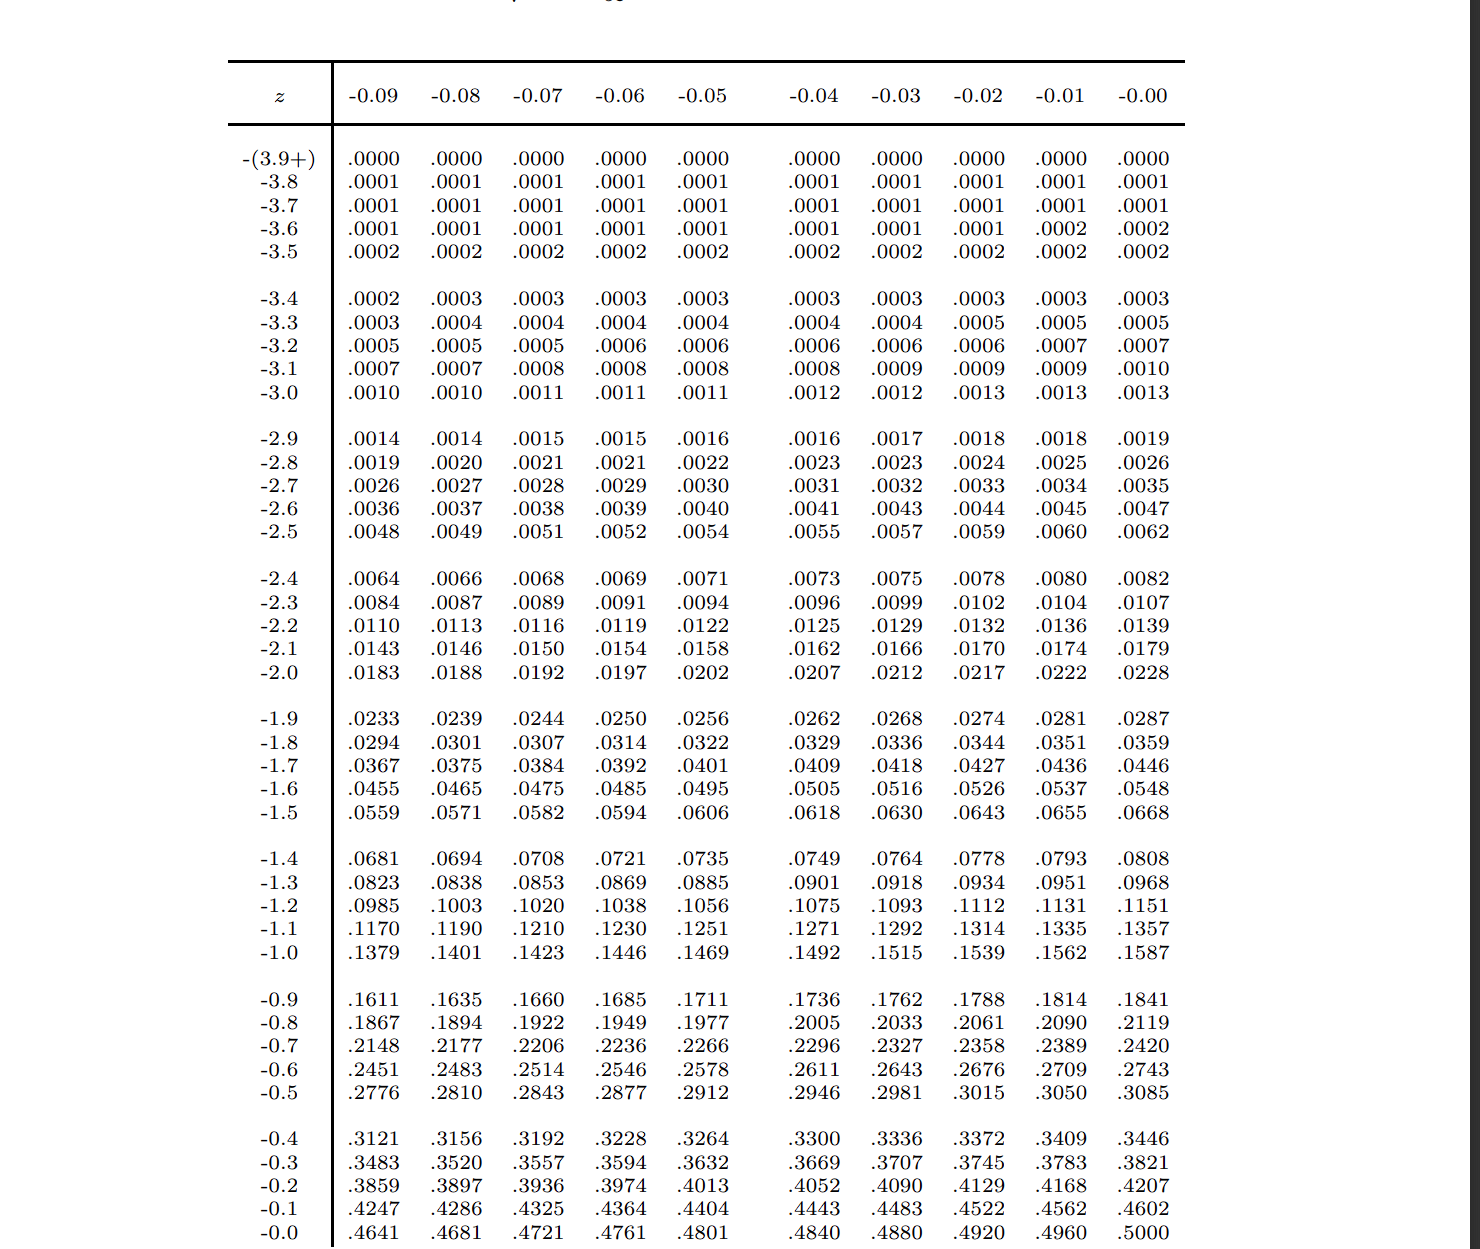
\includegraphics[width=1.3\textwidth]{nd1.png}
    \caption{Bảng phân phối chuẩn tắc 1}
    \label{fig:nd1}
\end{figure}

\begin{figure}[ht]
    \centering
    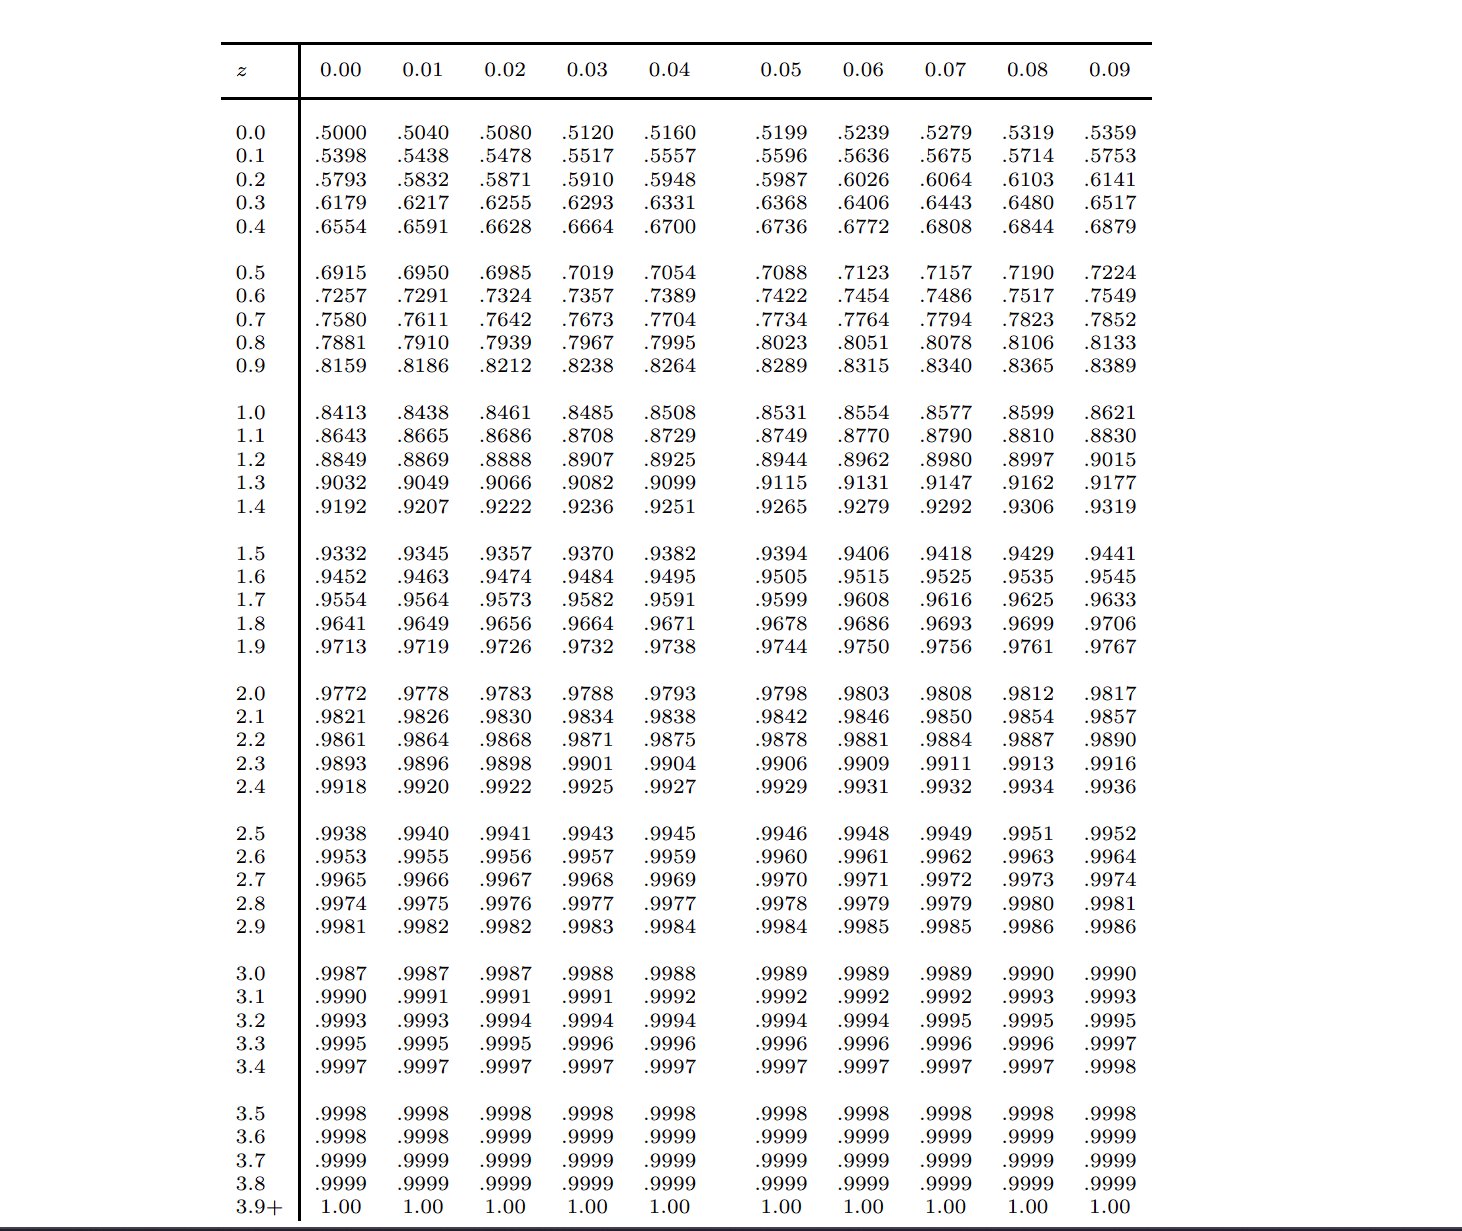
\includegraphics[width=1.3\textwidth]{nd2.png}
    \caption{Bảng phân phối chuẩn tắc 2}
    \label{fig:nd2}
\end{figure}

\end{document}